\documentclass[11pt]{article}
\usepackage[utf8]{inputenc}
\usepackage{amsmath,amsthm,amsfonts,amssymb,amscd}
\usepackage{multirow,booktabs}
\usepackage[table]{xcolor}
\usepackage{fullpage}
\usepackage{lastpage}
\usepackage{enumitem}
\usepackage{fancyhdr}
\usepackage{mathrsfs}
\usepackage{wrapfig}
\usepackage{setspace}
\usepackage{calc}
\usepackage{multicol}
\usepackage{cancel}
\usepackage[retainorgcmds]{IEEEtrantools}
\usepackage[margin=3cm]{geometry}
\usepackage{amsmath}
\newlength{\tabcont}
\setlength{\parindent}{0.0in}
\setlength{\parskip}{0.05in}
\usepackage{empheq}
\usepackage{framed}
\usepackage[most]{tcolorbox}
\usepackage{xcolor}
\colorlet{shadecolor}{orange!15}
\parindent 0in
\parskip 12pt
\geometry{margin=1in, headsep=0.25in}
\theoremstyle{definition}
\newtheorem{defn}{Definition}
\newtheorem{reg}{Rule}
\newtheorem{exer}{Exercise}
\newtheorem{note}{Note}

\usepackage[nottoc,notlot,notlof]{tocbibind}

\usepackage[superscript,biblabel]{cite}
\usepackage{hyperref}
\hypersetup{colorlinks,linkcolor={blue},citecolor={blue},urlcolor={orange}}

\usepackage{graphicx}
\usepackage[lofdepth,lotdepth]{subfig}
%Path relative to the main .tex file
\graphicspath{ {./images/} }

\title{\textbf{Heart rate variability analyzer}}
\author{
  Russel Shawn Dsouza\\
  171EC143
  \and
  Sathvik S Prabhu\\
  171EC146
}
\date{13 November, 2019}


\begin{document}
  \maketitle
  \thispagestyle{empty}
  % TODO Change titlepage to add logo

  \newpage
  \tableofcontents
  \thispagestyle{empty}

  \setcounter{page}{1}
  \newpage
  \begin{center}
    \large{\textbf{Abstract}}\\
    A portable, low power and low cost system is proposed to detect the heart rate variability features from a recorded ECG signal.
    The ECG is recorded with the help of the AD8232 signal condidtioning unit from where it is sent to an Arduino Uno.
    The signal data is then serially transmitted to a Raspberry Pi which handles the signal processing tasks. After filtering and normalization of the ECG, a peak detection algorithm is used to identify peaks. Based on this, various heart rate variability indices including the mean RR interval duration, standard deviation of RR intervals, RMS value of the successive differences of RR intervals, number of pairs of successive RR intervals that differ by more than 50 ms are extracted from the signal. The plots of the peaks detected, heart rate variation and the Poinare plot are then displayed on a monitor. The heart rate variability features can be used by physicians for during the diagnosis of different heart related disorders. These features can also be used for more complicated tasks like identification of stress level or detection of cardiac arrhythmia. More accurate sensors or  multiple sensors which record different physiological signals can be used together to improve and give a more holistic view during diagnosis of various disorders.

    \textbf{Keywords:} peak detection, Raspberry Pi, heart rate variablity, Poincare plot, Arduino
  \end{center}

  \section{Introduction}
  Electrocardiography (ECG or EKG) is a representation of the electrical activity of the heart as it changes with time. It is a plot of voltage, which is usually expressed in millivolts (mV), against time in seconds (s). This measurement is taken by placing electrodes on the skin at different points of the body. The analysis of ECG is done by physicians to assess various abnormalities associated with the heart and other cardiac functions. The heart rate variability (HRV) is a broad term given to the cycle to cycle variation in the ECG.

  The study and analysis of short-term and long-term variability in heart rate reflects the functioning of the vagal nerve and the sympathetic function of the autonomic nervous system, respectively.
  Heart rate variability can therefore be not only used as a monitoring tool in the diagnosis of cardiac ailments but also in clinical conditions with altered autonomic nervous system function.
  n diabetic patients, low heart rate variability is associated with an increased risk for sudden cardiac death.
  In neurologic disorders such as brain damage, the Guillain-Barre syndrome and uremic neuropathy, heart rate variability analysis can provide insight into which division of the autonomic nervous system is most affected.
  The analysis of the effects of drugs can also be studied using heart rate variability as it can also shed light on the mode of action of drugs.

  A typical ECG signal is characterized by a P wave, a QRS complex consisting of Q,R and S waves and a T wave as shown in figure \ref{fig:pqrst}.
  The automatic detection of the QRS complex or the R peaks in a long term electrocardiogram (ECG) signal is one of the most important steps in the diagnosis of cardiac disorders, biometric and ECG coding systems.

  \begin{figure}[h]
    \centering
    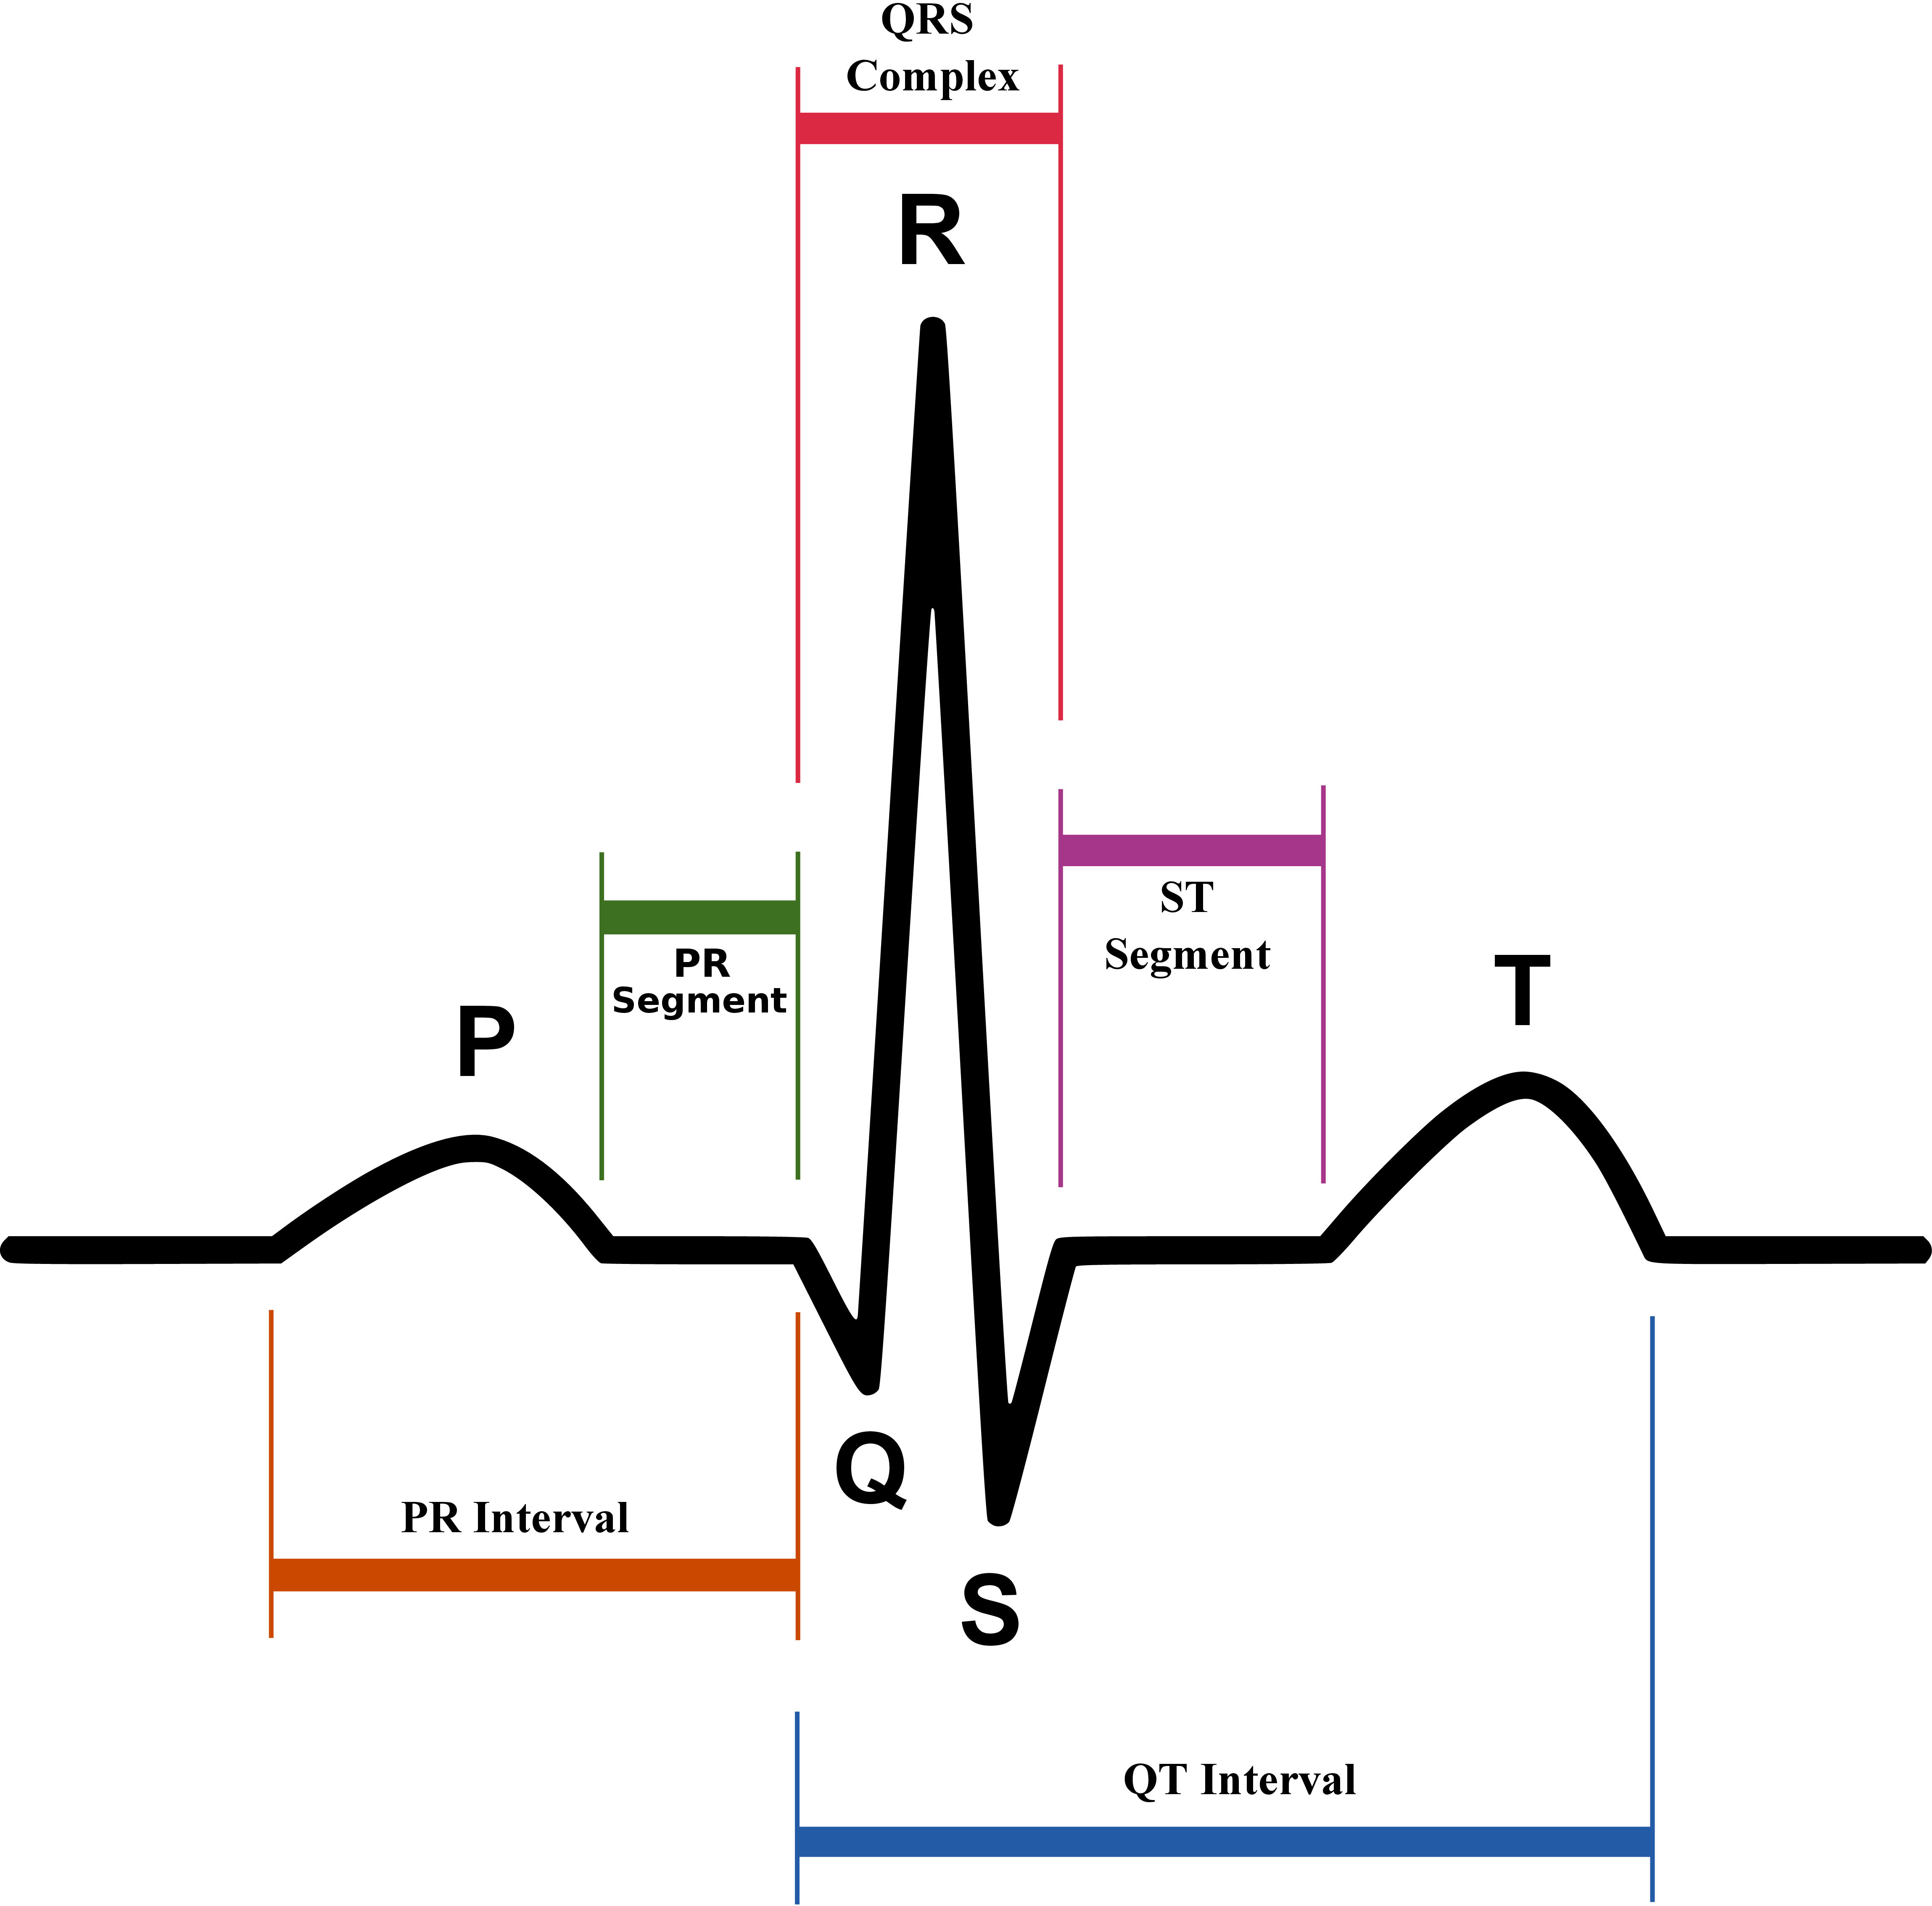
\includegraphics[scale=0.2]{images/SinusRhythmLabels.jpg}
    \caption{A typical ECG wave showing the P wave, QRS complex and S, T waves\cite{wiki:SinusRythmLabels}}
    \label{fig:pqrst}
  \end{figure}

  The P wave represents atrial depolarisation, or the contraction of the two atria.
  The PR interval indicates the time taken for the electrical impulse to reach the ventricles from the atria.
  The QRS complex represents the depolarisation of the ventricles.
  The RT interval denotes the time between depolarisation and repolarization or contraction of the ventricles.
  The T wave, which can be seen as a small wave after the QRS complex, represents ventricular repolarisation.
  The RR interval starts at the peak of one R wave and ends at the peak of the next R wave. It represents the time between two QRS complexes.

  \subsection{Motivation}
  In recent years, cardiac diseases have drawn great attention as they are the leading cause of mortality in developed countries.
  Long term monitoring of electrocardiogram (ECG) is therefore widely used for those with cardiac ailments.
  Many hardware systems have been proposed for ECG monitoring, which can be differentiated into recording and analyzing systems.

  A typical recording system mainly implements the processes of ECG signal acquisition, storage, and transmission.
  The analyzing system extracts the features from the ECG signal and sends it for analysis.
  Hence, it is necessary to design a joint system for both ECG recording and analyzing of its features, for example, its heart rate variability. Implementing this kind of system involves multiple challenges.
  An energy limited system needs high energy efficiency to prolong its service life.
  In the era of IoT, it is necessary to implement a pocket friendly method which is both portable and convenient.


  \section{Survey of the state of the art}
  Paulo et. al.\cite{melillo2011nonlinear} have used nonlinear features of HRV for automatically detecting real-life stress conditions. Features such as the approximate entropy, correlation dimesnion, fluctuation Analysis, recurrence Plot and the poincare plot were used along with the linear discriminant analysis (LDA) classifier to detect the stress level.

  Christov et. al. \cite{christov2018ranking} studied and ranked the most reliable heart rate variability features for the detection of atrial fibrillation in single-lead ECG. The identified features were the proportion of RR intervals differing by more than 50 ms from the preceding RR interval, Poincare plot geometry estimated by the ratio of the minor-to-major semi-axes of the fitted ellipse, P-wave presence in the average beat, the mean percentage of the RR interval first differences and the mean correlation of all beats against the average beat.

  Ni et. al.\cite{ni2019multiscale} have proposed a method to recognize the severity of hypertension using HRV features. They extracted 18 HRV multidimensional features in the time, frequency, and nonlinear domain. Then the temporal pyramid pooling method was designed to reduce feature dimensions. Multifactor analysis of variance (MANOVA) was later applied to filter the related features and establish the hypertension recognizing model with relevant features to efficiently recognize the patients’ severity.

  Low heart rate variability (HRV) has been demonstrated to be a major risk factor leading to various conditions, particularly cardiovascular disorders\cite{kamath1987heart}.
  On the other hand, high HRV has been shown to be an indicator of improved executive functions, such as attentional processing or impulse control\cite{appelhans2006heart, thayer2005psychosomatics}.
  High HRV has also been observed in different psychological conditions associated with symptoms of impaired behavioral and emotional regulation\cite{thayer2009claude, schulz2008negative}.


  \section{Features we wish to implement}
  \begin{itemize}
    \item \textbf{ECG Signal acquisition:} The ECG signal is obtained with the help of the sensor pads and the AD8232 unit.
    \item \textbf{Filtering and Pre-processing:} On the Raspberry Pi, the ECG signal is filtered and smoothened.
    \item \textbf{Detection of peaks}: A threshold based peak detection algorithm is applied to detect peaks.
    \item \textbf{Extracting features}: Time domain features are extracted after peak detection.
    \item \textbf{Plots}: The ECG peaks, change in heart rate and Poincare plots are displayed on the monitor along with the feature values.
  \end{itemize}

  \section{Implementation}
  \underline{Three sensor pads} are placed on specific regions of the body based on the concept of Einthoven’s triangle\cite{abi2019einthoven}, which is an inverted equilateral triangle as shown in figure \ref{fig:eithoven_triangle}. The voltages at these points give a net potential of zero, making the electrode setup electrically equilateral.

  \begin{figure}[h]
    \centering
    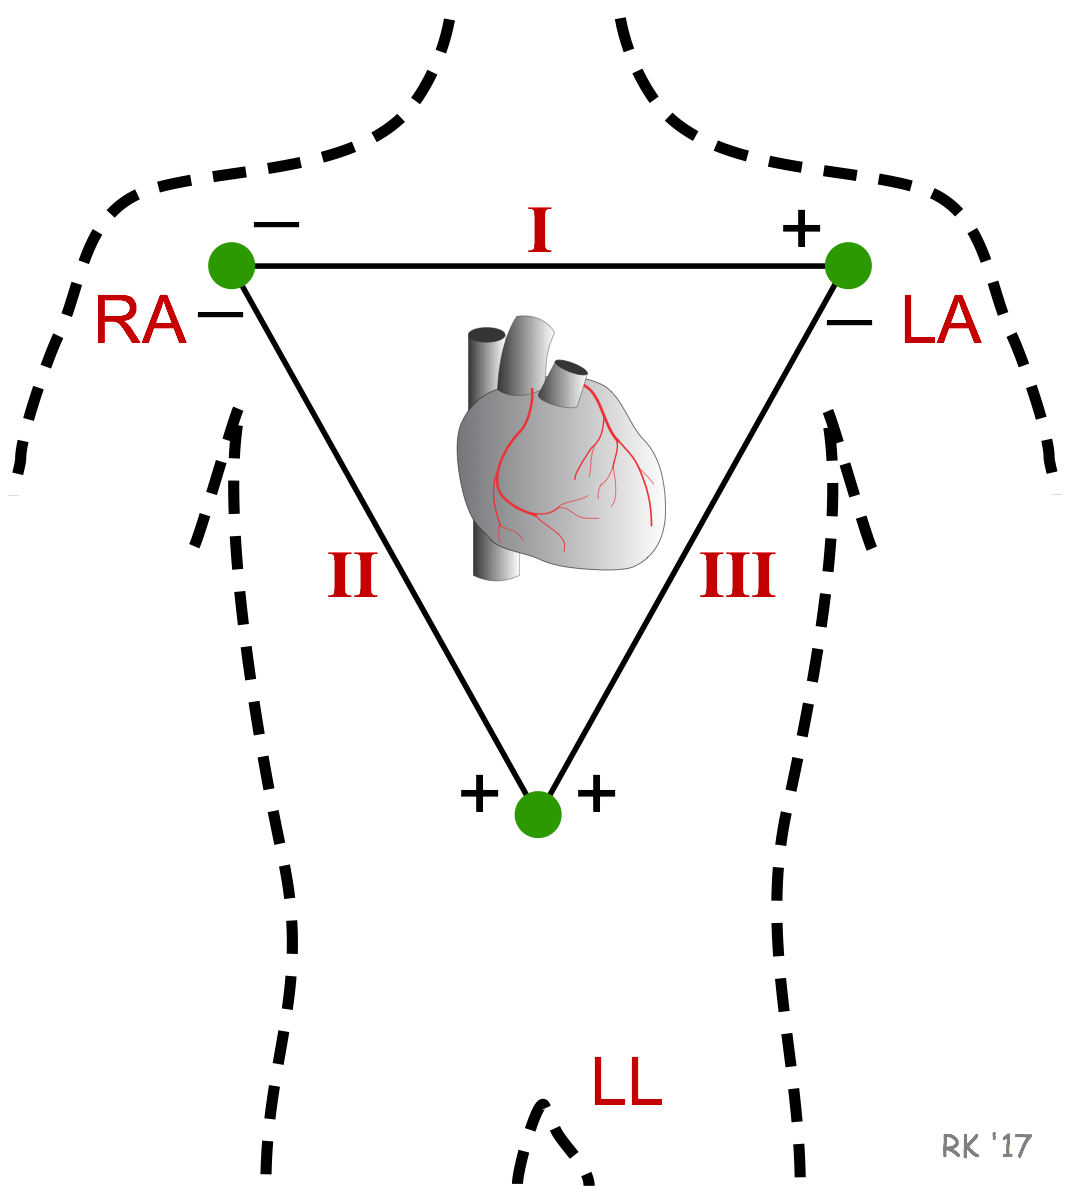
\includegraphics[scale=0.1]{images/eithoven_triangle.png}
    \caption{Eithoven's triangle\cite{cvp:ECG_eithoven}}
    \label{fig:eithoven_triangle}
  \end{figure}

  \underline{AD8232}\cite{ae:ad8232} module which is an integrated signal conditioning block for ECG and other biopotential signals.
  It is designed to extract, amplify, and filter small biopotential signals in the presence of noisy conditions, such as those created by motion or remote electrode placement.
  Its design allows it to be used as a part of low power and low cost applications.
  The AD8232 can implement a two-pole high-pass filter for eliminating motion artifacts.
  After an abrupt signal change that rails the amplifier (such as a leads off condition), the AD8232 automatically adjusts to a higher filter cutoff.
  This feature allows the AD8232 to recover quickly, and therefore, to take valid measurements soon after connecting the electrodes to the subject.

  \underline{Arduino Uno} used to record the data from the AD8232 at a fixed sampling rate, say 100 Hz.
 The data is then serially transmitted to the Raspberry Pi which can handle more complex processes using more computing power.   The Arduino handles the interfacing and collection of signal data and the Raspberry Pi focuses on the more power intensive tasks like signal processing and machine learning, if any.

  A \underline{Raspberry Pi 3B+} is used to process and analyse the signals.
  Short segments of ECG signals are taken and filtered, smoothened and normalized.
  A Peak detection algorithm is applied and then features are extracted from the RR durations in an ECG signal, where RR represents the period between two consecutive R peaks.
  On the Raspberry Pi, a Jupyter Notebook can be used to provide an interactive environment for signal processing and plotting different waveforms and graphs.

  The peak detection algorithm has been tested on the MAHNOB-HCI\cite{lichtenauer2011mahnob} dataset. Here, small ECG segments of length 10-20 seconds are first preprocessed and normalized. Then a threshold is determined in such a way that all peaks occur above this threshold. Finally the maximum point in each of these local segments are determined to find the peaks.

  \begin{figure}
    \centering
    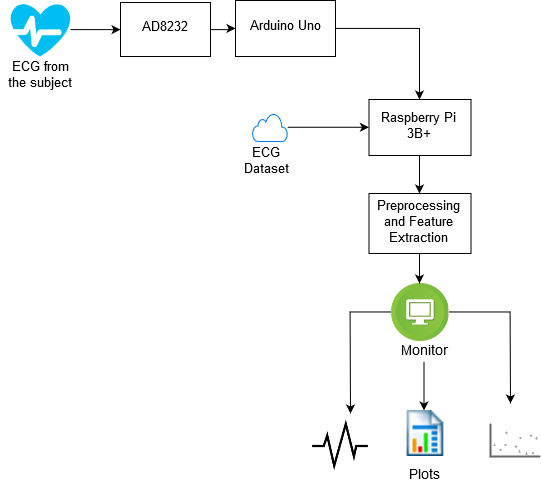
\includegraphics[width=0.5\textwidth]{images/block_diagram}
    \caption{Block schematic of the system}
  \end{figure}

  Features extracted include:
  \begin{itemize}[topsep=1pt]
    \item[] \textit{Mean RR} gives the average value of the RR duration in an ECG segment. This can be used to calculate the average heart rate (HR).
    \item[] \textit{SDNN} is the standard deviation of the NN (R-R) intervals
    \item[] \textit{RMSSD} is the root mean square of the successive differences of RR intervals, used for a good snapshot of the Autonomic Nervous System’s Parasympathetic branch and is the basis of the HRV Score.  RMSSD is considered as one of the most relevant and accurate measures of autonomic Nervous system activity over the short-term.
    \item[] \textit{NN50} is the number of pairs of successive NN (R-R) intervals that differ by more than 50 ms
    \item[] \textit{PNN50} is the proportion of NN50 divided by the total number of NN (R-R) intervals
    \item[] \textit{Poincare Plot} is graphed by plotting every R–R interval against the prior interval, creating a scatter plot.
    Poincare plot analysis allows researchers to visually search for patterns buried within a time series.
    The analysis of this plot is a geometrical and nonlinear method to assess the dynamics of HRV.
    The degree of heart failure can be evaluated quantitatively through the computation of the standard deviation (SD) indexes of the plot\cite{hsu2012poincare}.
  \end{itemize}

  \section{Results}
  The values of the various features obtained from a sample of the recorded ECG signal are tabulated.

  \begin{figure}
    \centering
    \subfloat[Subfigure 1 list of figures text][Raw Dataset ECG]
    {
    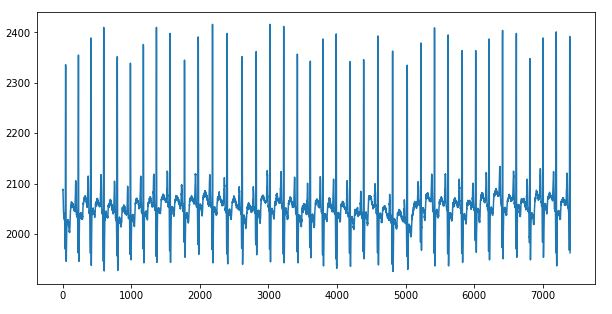
\includegraphics[width=0.4\textwidth]{ecg_raw}
    \label{fig:subfig1}
    }
    \qquad
    \subfloat[Subfigure 2 list of figures text][Dataset ECG after preprocessing]
    {
      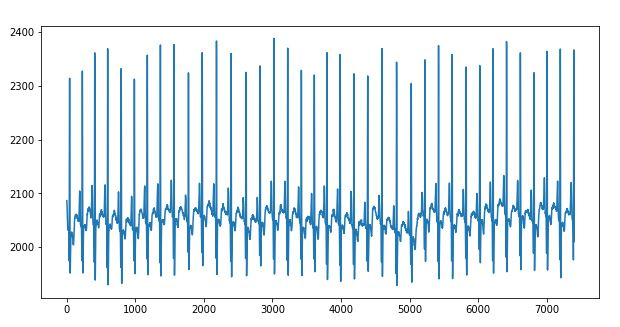
\includegraphics[width=0.4\textwidth]{ecg_averaged}
      \label{fig:subfig2}
    }
    \qquad
    \subfloat[Subfigure 3 list of figures text][Peak detection on Dataset ECG]
    {
      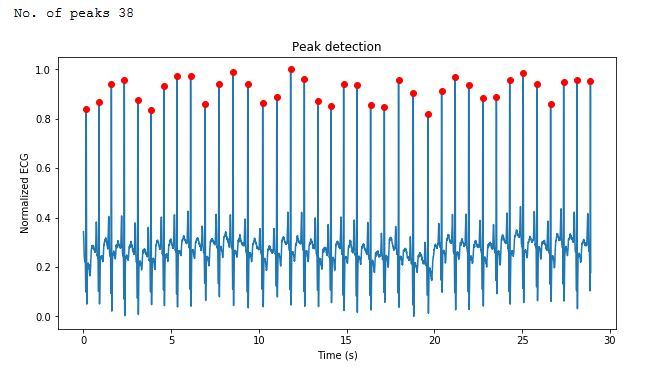
\includegraphics[width=0.4\textwidth]{ecg_peaks}
      \label{fig:subfig3}
    }
    \qquad
    \subfloat[Subfigure 4 list of figures text][Peak detection on recorded ECG]
    {
      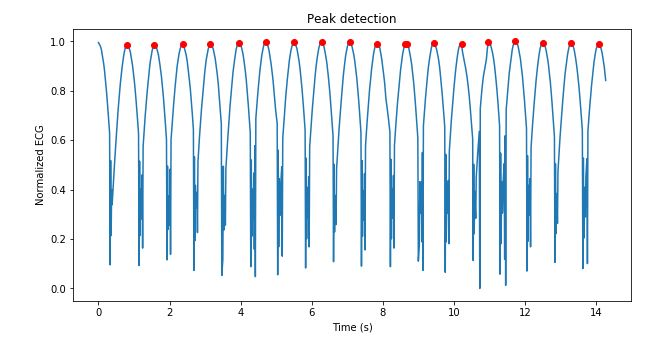
\includegraphics[width=0.4\textwidth]{ecglab_peaks}
      \label{fig:subfig4}
    }
    \caption{Processing of the ECG signal}
    \label{fig:globfig1}
  \end{figure}

  \begin{center}
    \begin{tabular}{|c | c |}
      \hline
      \textbf{Feature} & \textbf{Value}  \\
      \hline\hline
      Average HR & 77.4243  \\
      \hline
      SDNN & 0.0336 \\
      \hline
      RMSDD & 0.0259  \\
      \hline
      NN50 & 2.0000  \\
      \hline
      PNN50 & 0.0541  \\ [1ex]
      \hline
    \end{tabular}
    %\caption{Feature values for an ECG sample}
    %\label{table:1}
  \end{center}

  \begin{figure}
    \centering
    \qquad
    \subfloat[Subfigure 5 list of figures text][HR of Dataset ECG]
    {
      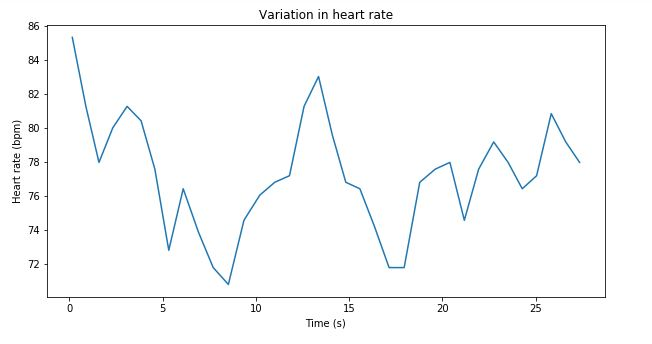
\includegraphics[width=0.4\textwidth]{ecg_hrv}
      \label{fig:subfig5}
    }
    \qquad
    \subfloat[Subfigure 6 list of figures text][HR of recorded ECG]
    {
      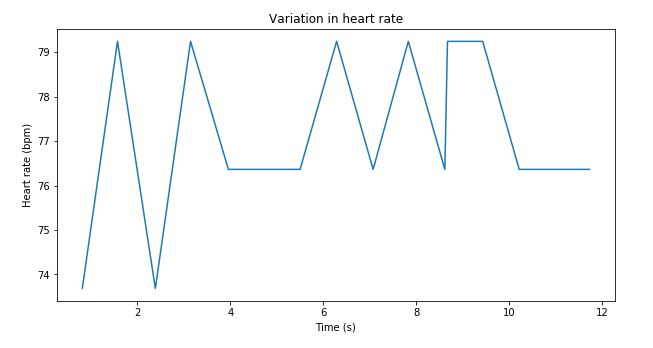
\includegraphics[width=0.4\textwidth]{ecglab_hrv}
      \label{fig:subfig6}
    }
    \qquad
    \subfloat[Subfigure 7 list of figures text][Poincare plot of Dataset ECG]
    {
      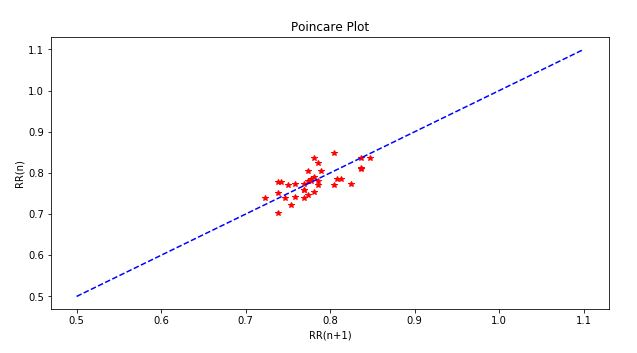
\includegraphics[width=0.4\textwidth]{ecg_poincare}
      \label{fig:subfig7}
    }
    \qquad
    \subfloat[Subfigure 8 list of figures text][Poincare plot of recorded ECG]
    {
      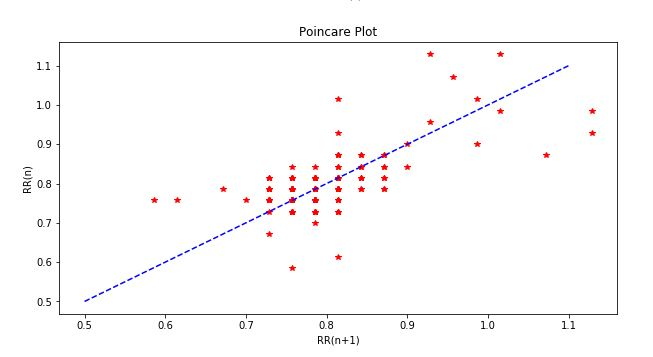
\includegraphics[width=0.4\textwidth]{ecglab_poincare}
      \label{fig:subfig8}
    }
    \caption{Plots obtained}
    \label{fig:globfig2}
  \end{figure}


  \newpage
  \section{Conclusion}
  A portable, low power and low cost system is implemented to record ECG signals from the subject and display the heart rate variability features. These features can be used by physicians during the diagnosis of heart related ailments or even a few neuro-physiological disorders. The accuracy of the features can be improved by using sensors which give better accuracy using which the more intricate features of the signal can be extracted.

  These features can also be used for other tasks like emotion recognition or detection of cardiac arrhythmia. One can use multiple sensors which record various signals from the body and extract features from different signals. These features can be then processed, maybe using an artificial neural network, for more complex tasks which require a more holistic view of things.

  In this era of IoT (Internet of Things), a bigger ecosystem can be built where the signal data collected can be sent to a remote server, processed there and and then the results can be accessed by the end user through a mobile app.



  \newpage
  \bibliography{bibliography}
  \bibliographystyle{ieeetr}
\end{document}
